\documentclass{article}  % this line must be in main document!! otherwise compiler gets confused

\usepackage[utf8]{inputenc}
% \usepackage{natbib}
\usepackage{physics}
\usepackage{biblatex}
\usepackage[hidelinks]{hyperref}

\usepackage[table,xcdraw]{xcolor}
\usepackage{svg}
\usepackage[T1]{fontenc}
\usepackage{amsmath}
\usepackage{amssymb}
\usepackage{dsfont}
\usepackage{lmodern}
\usepackage{units}
\usepackage{icomma}
\usepackage{graphicx}
\usepackage{eurosym}
\usepackage{verbatim}
\usepackage[margin=3.4cm]{geometry}
\usepackage{float}
\usepackage{listings}
\usepackage{mathtools}
\usepackage{caption}
\usepackage{color} %red, green, blue, yellow, cyan, magenta, black, white
\definecolor{mygreen}{RGB}{28,172,0} % color values Red, Green, Blue
\definecolor{mylilas}{RGB}{170,55,241}
\setcounter{MaxMatrixCols}{30}
\definecolor{dkgreen}{rgb}{0,0.6,0}
\definecolor{gray}{rgb}{0.5,0.5,0.5}
\definecolor{mauve}{rgb}{0.58,0,0.82}
\usepackage{textcomp}
\usepackage[titletoc,title]{appendix}
\DeclareMathOperator*{\argmax}{arg\,max}
\DeclareMathOperator*{\argmin}{arg\,min}
\allowdisplaybreaks
%
\lstset{language=Matlab,%
    %basicstyle=\color{red},
    breaklines=true,%
    morekeywords={matlab2tikz},
    keywordstyle=\color{black},%
    morekeywords=[2]{1}, keywordstyle=[2]{\color{black}},
    identifierstyle=\color{black},%
    stringstyle=\color{mylilas},
    commentstyle=\color{mygreen},%
    showstringspaces=false,%without this there will be a symbol in the places where there is a space
    numbers=left,%
    numberstyle={\tiny \color{black}},% size of the numbers
    numbersep=9pt, % this defines how far the numbers are from the text
    emph=[1]{for,end,break},emphstyle=[1]\color{black}, %some words to emphasise
    %emph=[2]{word1,word2}, emphstyle=[2]{style},    
}
\newcommand{\innerprod}[2]{\langle #1, #2 \rangle}
\addbibresource{bibliography.bib}

\title{TFR Notes}
\author{Veronika Chronholm}
\date{\today}

\begin{document}

\setcounter{secnumdepth}{2}
\pagestyle{plain} % stile pagina (header, numerazioni)

% \centerline {\includegraphics[width=2cm]{logo.jpg}}
\begin{center}
    \large{EPSRC Centre for Doctoral Training in Statistical Applied Mathematics (SAMBa)} \\
	\line(1,0){450}\\ 
	\vspace{3.5cm} 
	{ \huge \textbf{Numerical Methods for Radiation Transport and Radiotherapy Treatment Planning} \\}
	%\vspace{0.1cm}
	%\line(1,0){450} \\
    \vspace{1.5cm} 
    \Large{Thesis Formulation Report} \\
    \vspace*{9cm}
    \Large{Veronika Chronholm} \\
    \vspace{0.7cm}
    \large{Supervised by Professor Tristan Pryer}
\end{center}

\thispagestyle{empty}

% \vspace*{5cm}
% {\hspace*{6cm} \large{{\begin{tabular}{ll}
% 			Written by Veronika Chronholm \\
%             \end{tabular}
% 	}}
% }
\newpage
\tableofcontents
\setcounter{page}{1}

\newpage

% 1. I think you should add a little more info on the physical background and include relevent references, Bortfeld for example.
% 2. How do you get to equation 1? It’s a jump to start there. More detail before.
% 3. I think there’s a typo in eqn 1
% 4. I think you could mention different a’s come from different energy models, Bragg Kleeman, for example.
% 5. Eqn 4 doesn’t specify norms, then if you do, norms aren’t defined until lower. Perhaps just write _X or something
% 6. Same with 15
% 7. Why might you choose different p values in 24? Also, does it make sense to have the ‘error bit’ in the same norm as the ‘regularisation bit’?
% 8. Isn’t assumption 1 asking b and sigma are Lipschitz continuous in y and continuous in t?
% 9. Assumption 2 and 4 corresponds to an asymptotic growth condition? Can you comment on why it’s needed?
% 10. Assumption 3 is quite strict, is there a weaker variant discussed in some reference?
% 11. I think you can make 52 clearer if you write for x\in \Omega and t \in [0,T] after the equations and slap the ICs together with the PDEs
% 12. You need to mention something about convergence of the iterative scheme, reference the Kelley book
% 13. above 58 approcimate, run a spell checker
% 14. You should include the truncation errors in 58-62 or mention them somewhere and reference
% 15. what motivates the semi implicit temporal discretisation 63?
% 16. does 76 not just mean 0 < 1? Is the scheme unconditionally stable?


% \section{Notes/To Do}
% Things to write:
% \begin{itemize}
%     \item Background: introduce application to radiotherapy treatment planning and equations describing radiation transport. Introduce the simplified model (like reading course model) that we will focus on here. Maybe also full Boltzman equation?
%     \item Explain how the choice of norm for the minimisation problem can lead to nonlinear PDEs - this motivates use of the full FBSDE framework (because we get nonlinear source terms)
%     \item Explain why the full coupled system can't be fit into the FBSDE framework - the forward/primal equation is not of the form in the FBSDE system (even with constant coefficients, because of time reversal?)
%     \item Details of how $z$ gets its BCs and TC from those we have for $u$
%     \item Convergence of approximation (twofold x 2): Does the iterative scheme converge when soln's to the sequence of PDEs are exact? I.e. $u^{(k)} \rightarrow u^{(*)}$? And is $u^{(*)}$ the right thing? Furthermore, does the iterative scheme converge (and to the right thing) when the soln's to the sequence of PDEs are approximated numerical sol'ns?
%     \item Results of numerical experiments
%     \item Future extensions of this model/framework: Model for radiation in multiple spatial dimensions (now just 1D), better/more accurate discretisation schemes e.g. SSP, MLMC, higher order in general?
%     \item another future work thing: figure out how to parallelize the MC code?
%     \item Motivation for the SSP methods for FBSDE: iterating through numerically solving each PDE in sequence, we want to make sure error is not propagated / does not grow? (Also motivation for FBSDE framework is to deal with the nonlinearity that arises when a different norm is chosen for the optimisation problem)
%     \item Write about how BCs on the dual ($z$) are implemented in the Monte Carlo simulations + FC for boundary value problems (integration bound = stopping time, i.e. random!)
% \end{itemize}

% NB: Need more references: 

% \begin{itemize}
%     \item Ref for the PDE constrained optimisation problem (and the iterative scheme for $(u^{(k)},z^{(k)})$) needed
%     \item Reuse refs from reading course report 
%     \item Some ref for physics-y bits? Or medical bits?
%     \item We have a few refs for Monte Carlo stuff e.g. Gobet, Oksendal, Klebaner
%     \item Also the SSP FBSDE paper (already in refs here)
% \end{itemize}

\section{Introduction}
% \begin{itemize}
%     \item Introduce context and motivation 
%     \item Describe structure of report
% \end{itemize}

% \begin{itemize}
%     \item Motivation: radiotherapy treatment 
%     \item ((Different kinds of radiation (and how they interact with matter) ))
%     \item Maybe some maths / intro explanantion of problem formulation and description of eqn for radiation behaviour?
% \end{itemize}

Proton beam therapy is a type of radiotherapy treatment for cancer, which uses a ray of proton radiation to damage the tumour. The radiation deposits energy in the tissue, which causes DNA damage, stopping the tumour cells from replicating. Since radiation will also damage the DNA in non-tumour cells, it is also important to as far as possible spare the healthy tissue surrounding the tumour. This becomes even more important if the tumour is located near a vital organ. 

The amount of radiaton that the tumour and surrounding tissue are exposed to is measured in terms of energy deposited per unit length, or depth inside the tissue. This is also known as dose. The ways that protons interact with matter mean that they deposit very little energy when moving at high velocities, and deposit a lot of their energy when moving at lower velocities, resulting in further slowing down. As a result of this, the depth-dose profile for proton radiation has a sharp peak, where most of the energy is deposited \cite{newhauser2015physics}. By varying the starting velocities and directions of the incident proton beams, it is possible to produce a spread-out Bragg peak, which can cover the entirety of a tumour whilst delivering a significantly lower dose to the surrounding tissue, and a virtually zero dose at a larger depth than the far end of the spread-out peak. 

In addition providing an introduction to the physics behind proton therapy \cite{newhauser2015physics} also provides an overview of the history of proton therapy. The practice was first proposed in \cite{wilson1946radiological}, which suggested that, as higher energy particle accelerators for protons (amongst other particles) were becoming available, protons should be considered as an option for radiation beam therapy. Before it was possible to accelerate protons to high enough velocities, they would not have been a suitable choice for beam therapy, as protons with lower energies were not be able to travel far enough into the tissue. In \cite{bortfeld1997analytical}, a closed form analytical approximation of the Bragg curve valid for protons with energies in a range suitable for proton beam therapy (10 - 200 MeV) is derived. The Bortfeld model gives an approximation of the Bragg peak produced by a proton pencil beam, and is in good agreement with experimental observations for the given range of proton energies. 

In this report, we present a simple PDE model for radiation transport, which captures the key behaviour of proton radiation, and connect this model to an SDE model, which stochastically models the behaviour of individual protons. Using the PDE model, we formulate the problem of treatment planning mathematically as a PDE constrained optimisation problem. After treating the optimisation problem using the method of Lagrange multipliers, we introduce an iteartive scheme for solving the resulting coupled PDE system. Having introduced the theory of Feynman-Kac formulae yielding probabilistic representations of the solutions to certain PDEs, we then suggest a numerical approach which involves iteratively solving each of the coupled PDEs. We conduct some initial numerical experiments, implementing the iterative procedure in combination with a finite difference schem for one of the coupled PDEs, and a Monte Carlo simulation solution technique for the other. Finally, we outline a number of potential directions for future work.
% \section{Background}
\begin{itemize}
    \item Motivation: radiotherapy treatment 
    \item ((Different kinds of radiation (and how they interact with matter) ))
    \item Maybe some maths / intro explanantion of problem formulation and description of eqn for radiation behaviour?
\end{itemize}
\section{Theory}
A lot of this is already written below.
\begin{itemize}
    \item Derivation of coupled PDE system from constrained optimisation problem 
    \item Relevant Feynman-Kac formulae 
    \item Extension to different norm for optimisation problem + relation of resulting eqns to nonlinear Feynman-Kac formulae
    \item ((Why does $z$ work in MC framework but not $u$?))
    \item Motivation for hybrid methods: it's not been done before, and not for this application. Idea: speed up treatment planning! 
    \item FC formulae for boundary value problems
    \item Add conditions for FC formulae to hold??
\end{itemize}

\subsection{Modelling radiation transport}
In this section, we describe a simple model for the evolution of radiation in a domain. Specifically, we are interested in approximately describing the behaviour of protons. On a microscopic level, as individual protons travel through space in a material, they interact with the atoms in the medium in a few different ways. These interactions govern the continuing movement of the protons, e.g. how their direction and speed of movement changes, and if and when they come to a stop inside the medium. Specifically, proton interactions with matter can be dividied into three categories. First, nonelastic collisions with the nuclei of the atoms in the medium and second, elastic scattering off of the nuclei. Third, we have inelastic Coulomb interactions between the protons and the electrons of the atoms in the medium, due to the positive charge of the protons and negative charge of the electrons. In the simplified model considered here, we capture the elastic scattering and the Coulomb interaction, but assume that the nonelastic collisions between protons and atomic nuclei happen rarely enough that we can ignore them. 

For simplicity we consider a one-dimensional domain in space. In this case, the radiation intensity $u(t,x,v)$ as a function of time $t$, position $x$, and velocity $v$ can be described by the PDE
%
\begin{align}
    \label{eq:pde-model}
    \partial_t u + v \partial_x u - \frac{\sigma^2}{2} \partial_v^2 - \partial_v \big( a(v) u\big) = g(t,x,v),
\end{align}
%
where the $\partial_x$ term describes transport through space, the $\partial_v$ term describes energy depletion, and the $\partial_v^2$ term describes the elastic scattering. The function $g$ is a source term, describing the input of additional radiation into the domain. 

Protons moving through a medium do not slow down linearly. Instead, they deposit very little energy when moving at high velocities, and much more when moving at low velocities, meaning that their velocities change more rapidly once they start slowing down. By choosing the function $a(v)$ to be a rapidly decreasing function of $v$, we are able to capture this behaviour in our model. For example, we might choose $a(v) = e^{-cv}$ for some constant $c$.

Another description of radiation transport can be formulated in terms of SDEs describing the evolution of the position $X_t$ and velocity $V_t$ of an individual proton, where $X_t$ and $V_t$ are Itô processes obeying the equations
%
\begin{align} 
    \label{eq:sde-model}
    X_t &= x_0 + \int_{0}^{t} V_s ds\\ 
    V_t &= v_0 - \int_{0}^{t} a(V_s) ds + \int_{0}^{t} \sigma dW_s.
\end{align}
%
In fact, in the case when $g=0$, the solution to \autoref{eq:pde-model} is the probability density function of $(X_t,V_t)$. In other words, we could think of \autoref{eq:pde-model} as describing the overall (macroscopic) behaviour of radiation through space, whilst \autoref{eq:sde-model} describes the (microscopic) behaviour of individual particles. In later subsections, we will discuss this type of connections between PDEs and SDEs, through so-called Feynman-Kac formulae, in more detail.

\subsection{Treatment planning as a PDE constrained optimisation problem}

% - PDE constrained optimisation problem 

% - Introduce our special case model

% - But, what norm do we use? Introduce Bochner spaces (and this particular one also has an inner product, which is important)

% - Write down the Lagrangian

% - Functional derivatives = zero yields three equations, which become the two coupled PDEs

% - Comment on how the problem would change if we changed the norm we're minimising in?

% - Radiotherapy: interested in the dose / energy deposited as a function of space/depth. Obtained by integrating $u$ over time and velocity.

% - Treatment planning: want to find the best way to give the desired dose to tumour (whilst sparing the surrounding area), and using as low an amount of radiation as possible whilst still reaching target dose on tumour --> PDE constrained optimisation problem 

% - For simplicity we consider a target radiation intensity instead of a target dose

% - Explain in more detail about PDE constrained optimisation

% - Explain in more detail the derivation of the Lagrangian maybe?

% - If we choose a different norm we get a different PDE - specifically a different source term in the dual equation


In the context of radiotherapy treatment, we are interested in the total amount of energy deposited as a function of depth in the tissue. This quantity is also called the radiation dose, and is obtained from the radiation intensity $u(t,x,v)$ by integrating over time and velocity. When treating a tumour, we want to expose the tumour to a sufficient dose of radiation, whilst sparing the healthy tissue surrounding the tumour as much as possible. We also want the total radiation exposure to be as low as possible, whilst still delivering a high enough dose to the tumour. 

We can formulate the task of treatment planning as a constrained optimisation problem, where we want to minimise the norm of the difference between the target dose and the achieved dose with a given source. The constraint consists of our PDE model describing the evolution of radiation intensity in the domain. To simplify the mathematical problem formulation, we will seek to minimise the difference between a target radiation intensity and the achieved radiation intensity.

As before, we let $u$ denote the radiation intensity in the domain. Letting $d_T$ denote the target intensity, we seek the radiation intensity $u$ and source $g$ that gives
%
\begin{align} 
    \label{eq:to-minimise}
    \min \frac{1}{2} {\lVert u - d_T \rVert}^2 + \frac{\alpha}{2} {\lVert g \rVert}^2
\end{align}
%
for some constant $\alpha$, and subject to the constraint
%
\begin{align}
    \label{eq:pde-constraint}
    &\partial_t u + \div{(\vecbf{b} u - \vecbf{A} \nabla u)} = g\\
    &{u \rvert}_{\partial \Omega} = 0\\
    & u(0,x,v) = f_0(x,v)
\end{align}
%
where 
%
\begin{equation}
    \vecbf{b} = 
    \begin{pmatrix}
        &v\\
        &-a(v)
    \end{pmatrix},
    \vecbf{A} = 
    \begin{pmatrix}
        &0 &0\\
        &0 &\frac{\sigma^2}{2}
    \end{pmatrix},
    \end{equation}
    %
so that we recover the PDE of \autoref{eq:pde-model}. We have also specified a zero boundary condition in $x$ and $v$, and a (potentially nonzero) initial condition $f_0(x,v)$. Since we are only considering one spatial dimension, our problem has a total of two dimensions in addition to time, i.e. $u(t,x,v): [0,T] \cross \Omega \rightarrow \mathbb{R}$ and the domain $\Omega=\mathbb{R}\cross\mathbb{R}$ is two-dimensional, with one dimension being position and the other velocity. We note that the constant $\alpha$ here functions as a regularisation parameter, whose value will need to be chosen appropriately for a numerical optimisation algorithm to converge. By chosing a larger $\alpha$, we penalise a large source $g$ more, whilst a smaller $\alpha$ corresponds to less of a penalty.

So far, we have formulated this optimisation problem without specifying which norm is used in \autoref{eq:to-minimise}. An intuitive choice may be the $L^2$ norm over the domain $\Omega$, but if we choose this norm we haven't taken into account the time dependence of $u$. With this in mind, we introduce the more general concept of a Bochner space $L^p(T;X)$ and the corresponding norm
%
\begin{align} 
    {\lVert (\cdot) \rVert}^p_{L^p(T,X)} := \int_{T} {\lVert (\cdot)\rVert}^p_X dt, 
\end{align}
%
where $X$ is a Banach space with corresponding norm ${\lVert \cdot\rVert}_X$. Specifically, we choose the case where $T$ is a time interval and $X=L^2(\Omega)$. A suitable choice for the norm for the minimisation problem \autoref{eq:to-minimise} is then the following;
%
\begin{align} 
    \lVert f \rVert_{L^2([0,T];L^2(\Omega))}^2 &:= \int_{0}^{T}  {\lVert f \rVert}^2_{L^2(\Omega)} dt\\
    &= \int_{0}^{T} \int_{\Omega} f^2 d\Omega dt.\\
\end{align}
%
We note that the space $L^2([0,T];L^2(\Omega))$ additionally has an inner product, namely
%
\begin{align} 
    \innerprod{f}{g}_{L^2(T;L^2(\Omega))} &:= \int_{0}^{T} \innerprod{f}{g}_{L^2(\Omega)} dt \\
    & = \int_{0}^{T} \int_{\Omega} fg d\Omega dt.
\end{align}
%
This inner product will be used in what follows.

We now proceed to treat the minimisation problem, using the method of Lagrange multipliers. First, we formulate the Lagrangian function for the optimisation problem specified by \autoref{eq:to-minimise} and \autoref{eq:pde-constraint}. Then, we take generalised derivatives of the Lagrangian function and set these to zero. Finally, from the resulting equations we obtain a set of two coupled PDEs.

Letting $\lVert \cdot \rVert$ and $\innerprod{\cdot}{\cdot}$ denote the norm and inner product in $L^2([0,T];L^2(\Omega))$, the Lagrangian function is given by
%
\begin{align} 
    \mathcal{L}(u,g,z) := \frac{1}{2} {\lVert u - d_T \rVert}^2 + \frac{\alpha}{2} {\lVert g \rVert}^2 - \innerprod{u}{\partial_t z} - \innerprod{u}{\vecbf{b} \cdot \nabla z} + \innerprod{\nabla u}{\vecbf{A} \nabla z} - \innerprod{g}{z}.
\end{align}
%
The function $u$ is the function that we seek in the minimisation problem, $g$ is the source term from the constraining PDE, and $z$ is another function known as the Lagrange multiplier, which is introduced to capture the constraint. 

By taking generalised (functional) derivatives of $\mathcal{L}$ with respect to $u$,$z$, and $g$ we obtain the following;
%
\begin{align} 
    D_u \mathcal{L}[\phi] &= \int_{0}^{T} \int_{\Omega} \Big((u-d_T)\phi - \partial_t z \phi - \phi \vecbf{b}\cdot\nabla z + \vecbf{A} \nabla z \cdot \nabla \phi \Big) d\Omega dt\\
    &= \int_{0}^{T} \int_{\Omega} \Big((u-d_T)\phi - \partial_t z \phi - \phi \vecbf{b}\cdot\nabla z + \div{(\vecbf{A} \nabla z)} \phi \Big) d\Omega dt,
\end{align}
%
\begin{align} 
    D_z\mathcal{L}[\phi] = \int_{0}^{T} \int_{\Omega} \Big( \phi \partial_t u + \div{(\vecbf{b}u)} \phi - \div{(\vecbf{A} \nabla u)} \phi - g \phi \Big) d\Omega dt,
\end{align}
%
\begin{align} 
    D_g\mathcal{L}[\phi] = \int_{0}^{T} \int_{\Omega} \Big( \alpha g \phi - z \phi \Big) d\Omega dt,
\end{align}
%
where $\phi = \phi(t,x,v) \in C^{\infty}_{0}$ is any test function which is infinitely continously differentiable and zero on the boundary of the integration domain.

By requiring $D_u \mathcal{L}[\phi]=D_z \mathcal{L}[\phi]=D_g \mathcal{L}[\phi]=0$ and applying the fundamental theorem of calculus of variations, we get a PDE for $z$;
%
\begin{align} 
    - \partial_t z - \vecbf{b} \cdot \nabla z - \div{(\vecbf{A} \nabla z)} + (u - d_T) = 0,
\end{align}
% 
a PDE for $u$;
%
\begin{align} 
    \partial_t u + \div{(\vecbf{b}u)} - \div{(\vecbf{A} \nabla u)} - g = 0,
\end{align}
%
which we note recovers the constraint \autoref{eq:pde-constraint}, and finally a relationship between $z$ and $g$;
%
\begin{align}
    \alpha g - z = 0. 
\end{align}
%
Putting these three equations together, we obtain the coupled PDEs 
%
\begin{align} 
    \label{eq:coupled-pdes}
    \begin{cases} 
        \partial_t u + \div{(\vecbf{b}u)} - \div{(\vecbf{A} \nabla u)} &= \frac{1}{\alpha} z\\
        \partial_t z + \vecbf{b} \cdot \nabla z + \div{(\vecbf{A} \nabla z)} &= u - d_T,
    \end{cases}
\end{align}
%
where the source term of the equation for $u$ depends on $z$, and vice versa.

The boundary condition ${u \rvert}_{\partial \Omega} = 0$ on $u$ is inherited by $z$. We can see that this is a sensible choice by considering the derivation of the weak formulation of the PDE obeyed by $u$.

In terms of boundary contidions in $t$, we have an initial condition on $u$; $u(0,x,v)=f_0(x,v)$ for some function $f_0(x,v)$ and a terminal condition on $z$; $z(T,x,v)=0$. The initial condition on $u$ and terminal condition on $z$ make it natural to solve $u$ forward in time and $z$ backward in time when considering the coupled problem numerically. We can see that imposing a zero terminal condition on $z$ makes sense by considering \autoref{eq:coupled-pdes}, and the case where $u=d_T$. In this case, if $z(T,x,v)=0$, the solution to the dual equation is given by $z(t,x,v)=0$, and $u$ solves the primal equation with a zero source term. 

We note that choosing a different norm for the optimisation problem would affect the form of \autoref{eq:coupled-pdes}. For example, we could choose to minimise the difference between $u$ and $d_T$ in the $L^p([0,T],L^p(\Omega))$-norm for some integer $p\neq 2$ instead. Specifically, we might then seek the $u$ and $g$ which minimise the expression 
%
\begin{align} 
    \frac{1}{p} {\lVert u - d_T \rVert}^p_{L^p([0,T],L^p(\Omega))} + \frac{\alpha}{p} {\lVert g \rVert}^p_{L^p([0,T],L^p(\Omega))}.
\end{align}
%
In this case, we would get the coupled PDEs 
%
\begin{align} 
    \label{eq:nonlinear-pde-system}
    \begin{cases} 
        \partial_t u + \div{(\vecbf{b}u)} - \div{(\vecbf{A} \nabla u)} &= {\Big(\frac{z}{\alpha} \Big)}^{\frac{1}{p-1}} \\
        \partial_t z + \vecbf{b} \cdot \nabla z + \div{(\vecbf{A} \nabla z)} &= {\big(u - d_T\big)}^{p-1},
    \end{cases}
\end{align}
%
where we note that both the primal and dual equation now have nonlinear source terms. 

In this report, we focus on the optimisation problem in the $L^2([0,T],L^2(\Omega))$-norm, where the resulting coupled PDEs are linear. However, we present this extension here, and cover some numerical methods for this general case in later sections, as a potential avenue for future work.

\subsection{Forward SDE and linear Feynman-Kac formula}

In this section, we delve into more detail regarding the connections that can be made between PDEs and SDEs through Feynman-Kac formulae. Here, we focus on the case of linear PDEs, whilst we cover nonlinear Feynman-Kac formulae in the following section. This treatment follows that of \cite{gobet2016monte}, where proofs of many of the stated formulae can be found. 

Let $b:\mathbb{R}^+ \times \mathbb{R}^d \rightarrow \mathbb{R}^d$, $\sigma:\mathbb{R}^+ \times \mathbb{R}^d \rightarrow \mathbb{R}^{d \times d}$, and $W_t$ a $d$-dimensional Brownian motion. Consider the $d$-dimensional SDE
%
\begin{align}
    \label{eq:gen-sde}
X_t = x + \int_0^t b(s,X_s) ds + \int_0^t \sigma(s,X_s)dW_s
\end{align}
%
describing the Itô process $X_t$. 

The infinitesimal generator of $X_t$ is the differential operator defined by 
%
\begin{align} 
    \mathcal{L}f(x) = \lim_{t\rightarrow 0} \frac{\mathbb{E}_x[f(X_t)]-f(x)}{t},
\end{align}
%
and is given by
%
\begin{align}
    \label{eq:generator-operator}
    \mathcal{L} = \frac{1}{2} \sum_{i,j=1}^d [\sigma \sigma^T]_{i,j}(t,x) \partial_{x_i,x_j}^2 + \sum_{i=1}^d b_i(t,x) \partial_{x_i}.
\end{align}
%

Below, we describe the connection between a PDE involving this differential operator, and the solution to the SDE \autoref{eq:gen-sde}, yielding a probabilistic representation of the solution to the PDE. We consider the terminal value problem
%
\begin{align}
    \label{eq:backward-pde}
    \begin{cases}
    &\partial_t u(t,x) + \mathcal{L}u(t,x) - k(t,x)u(t,x) + g(t,x) = 0, \quad t<T,x \in \mathbb{R}^d, \\
    &u(T,x) = f(x).
    \end{cases}
\end{align}
%
We note that the probabilistic convention is to formulate this problem as a terminal value problem, as we have done here. However, the PDE convention would be to instead formulate it as an initial value problem. These two formulations are equivalent under a time-reversal $t \mapsto T-t$, as is discussed in \cite{gobet2016monte}. 

Under some conditions on the functions $f, g, k$ as well as on $b$ and $\sigma$, and provided that the solution $u$ to \autoref{eq:backward-pde} exists and is sufficiently regular, we can represent $u(t,x)$ through a so-called Feynman-Kac formula. Specifically, the following conditions are sufficient:

\begin{enumerate}
    \item $b(t,x)$ and $\sigma(t,x)$ are continous functions satisfying the following conditions for some constant $C$: \begin{enumerate}
        \item $\lvert b(t,x) - b(t,y) \rvert + \lvert \sigma(t,x) - \sigma(t,y) \rvert \leq C \lvert x - y \rvert \quad \forall (t,x,y) \in [0,T]\cross \mathbb{R}^d \cross \mathbb{R}^d$
        \item $ \sup_{0\leq t \leq T} \lvert b(t,0) \rvert + \lvert \sigma(t,0) \rvert \leq C$
    \end{enumerate}
    \item The functions $f:\mathbb{R}^d \rightarrow \mathbb{R}$, $g,k : [0,T]\cross \mathbb{R}^d \rightarrow \mathbb{R}$ are all continuous and fulfill the following:
    \begin{align} 
        \sup_{x \in \mathbb{R}^d} \frac{\lvert f(x) \rvert}{1 + {\lvert x \rvert} ^2} + \sup_{0 \leq t \leq T, x \in \mathbb{R}^d} \frac{\lvert g(t,x) \rvert}{1 + {\lvert x \rvert}^2} + \lvert k(t,x) \rvert < + \infty.
    \end{align}
    \item The solution $u$ to the boundary value problem \autoref{eq:backward-pde} exists and is continously differentiable once in $t$ and twice in $x$.
    \item $u(t,x)$ is continous on the domain $[0,T]\cross\mathbb{R}^d$ and satisfies 
    \begin{align} 
        \sup_{0\leq t \leq T, x \in \mathbb{R}^d} \frac{\lvert u(t,x) \rvert}{1 + {\lvert x \rvert}^2} < + \infty.
    \end{align}
\end{enumerate}
In summary, condition 1 arrures the existence and uniqueness of the solution to the SDE \autoref{eq:gen-sde}, whilst conditions 2 and 4 are conditions on the growth of $f,g,k$ and $u$ respectively. Condition 3 dictates that the solution $u$ to the terminal value problem must exist and be sufficiently regular.

Provided that these conditions are fulfilled, $u(t,x)$ is given by the Feynman-Kac formula
%
\begin{align}
    \label{eq:linear-fc} 
    u(t,x) = \mathbb{E}\bigg[ f\big( X_T^{t,x} \big) e^{-\int_t^T k(r,X_r^{t,x})dr} + \int_t^T g(s,X_s^{t,x}) e^{-\int_t^s k(r,X_r^{t,x})dr}ds\bigg].
\end{align} 
%
Here $X_T^{t,x}$ denotes the stochastic process $X$ at time $T$, started at $x$ at time $t$. For a proof of this, see e.g. \cite{gobet2016monte}.

We have now formulated a probabilistic representation of \autoref{eq:backward-pde}, which is a terminal value problem, but exists in an infinite domain $\mathbb{R^d}$ in space. If we are instead considering the same PDE but on a bounded domain in space, we must also specify a boundary condition in $x$, and the probabilistic representation changes slightly.

Consider the boundary value problem
%
\begin{align}
    \label{eq:general-bvp}
    \begin{cases}
        &\partial_t u(t,x) + \mathcal{L}u(t,x) - k(t,x)u(t,x) + g(t,x) = 0, \quad t<T,x \in \Omega, \\
        &u(T,x) = f(T,x), \quad x \in \Omega \\ 
        &u(t,x) = f(t,x), \quad (t,x) \in [0,T[\cross \partial\Omega.
    \end{cases}
\end{align}
%
To write down its probabilistic representation we must first define the first exit time from the domain $\Omega$. The first exit time $\tau^{t,x}$ of the process $X^{t,x}$ (started at time $t$ at position $x$) from the domain $\Omega$ is given by $\tau^{t,x} = \inf{\{ s > t : X^{t,x}_s \notin \Omega \}}$. We note that the first exit time $\tau^{t,x}$ is a random variable -- if we consider different individual realisations of $X_s^{t,x}$, $\tau^{t,x}$ will take different values depending on the exact path of $X_s^{t,x}$. 

For the probabilistic representation of the solution to the boundary value problem \autoref{eq:general-bvp} to exist, the conditions listed above for the terminal value problem should be modified slightly. It is sufficient to require the following:

\begin{enumerate}
    \item The conditions on $b$ and $\sigma$ required for the existence and uniqueness of the solution to the SDE hold as above.
    \item The boundary $\partial \Omega$ of the spatial domain is smooth and it holds that 
    \begin{align} 
        \forall t \in [0,T], \forall x \in \partial \Omega, \quad \mathbb{P}(\tau^{t,x}=t) = 1, 
    \end{align}
    i.e. if the process $X^{t,x}$ is started at time $t$ at a point $x$ on the boundary of the domain, the first exit time $\tau^{t,x}$ is the starting time $t$.
    \item The functions $f,g,k : [0,T] \cross \Omega \rightarrow \mathbb{R}$ are continuous.
    \item The solution $u$ to the boundary value problem exists, is continous, and is continuosly differentiable once in $t$ and twice in $x$.
\end{enumerate}
We note that the growth conditions on $f,g,k$ and $u$ that were needed previously are not required in this case, where we have a bounded domain $\Omega$.

Denoting $\min{(t,s)} = t \wedge s$, the probabilistic representation of the solution to \autoref{eq:general-bvp}, which exists under the conditions listed above, is given by
%
\begin{align} 
    \label{eq:linear-fc-bvp}
    u(t,x) = \mathbb{E} \bigg[ &f\big(\tau^{t,x} \wedge T , X^{t,x}_{\tau^{t,x}\wedge T}\big) e^{-\int_t^{\tau^{t,x}\wedge T} k(r,X^{t,x}_r) dr}\\
    & + \int_t^{\tau^{t,x}\wedge T} g(s,X^{t,x}_s) e^{-\int_t^s k(r,X^{t,x}_r) dr} ds \bigg].
\end{align}
%
There are two main differences between this representation and \autoref{eq:linear-fc}. Firstly, the function $f(x)$ specifying the terminal condition has been generalised to a function $f(t,x)$ specifying both the terminal and boundary conditions. Secondly, anywhere the terminal time $T$ featured in the first formula, it has been replaced by the minimum of $T$ and the time $\tau^{t,x}$ at which $X^{t,x}$ first hits the boundary of the domain.

As it will prove useful later, we also write down a special case of \autoref{eq:linear-fc-bvp}, namely the case where $k=0$ and we also have a zero boundary and terminal condition, $f(t,x)=0$ for all $(t,x)$. In this case, the probabilistic representation of $u(t,x)$ is simply given by
%
\begin{align} 
    u(t,x) = \mathbb{E} \bigg[ \int_t^{\tau^{t,x}\wedge T} g(s,X^{t,x}_s) ds \bigg].
\end{align}
%
We note that the zero boundary condition on $u(t,x)$ corresponds to killing $X_s^{t,x}$ once it hits the boundary of the domain, $\partial \Omega$.

Finally, we make a connection betwen the SDE \autoref{eq:gen-sde} and another PDE, which describes the probability distribution of $X_s^{t,x}$, and sketch a possible Feynman-Kac representation of its solution. First, we note that a special case of \autoref{eq:linear-fc}, when $k=0,g=0$, gives the solution to the Kolmogorov backward equation (with terminal condition),
%
\begin{align}
    \label{eq:kolmogorov-backward}
    \begin{cases}
    &\partial_t u(t,x) + \mathcal{L}u(t,x) = 0, \quad t<T,x \in \mathbb{R}^d, \\
    &u(T,x) = f(x),
    \end{cases}
\end{align}
%
is given by 
%
\begin{align}
    u(t,x) = \mathbb{E}\big[ f(X_T^{t,x}) \big]. 
\end{align} 
% 
The adjoint of the Kolmogorov backward equation is the Kolmogorov forward equation
%
\begin{align} % sign?
    \label{eq:kolmogorov-forward}
    \partial_s p(s,y) - \mathcal{L}^{*}p(s,y) = 0,
\end{align}
%
where the differential operator $\mathcal{L}^{*}$ is the adjoint of $\mathcal{L}$, given by
%
\begin{align}
    \label{eq:adjoint-operator}
     \mathcal{L}^{*} = \frac{1}{2} \sum_{i,j=1}^{d} \partial_{y_i,y_j} [\sigma \sigma^T]_{i,j}(s,y) - \sum_{i=1}^{d} \partial_{y_i}b_i(s,y).
\end{align} 
%
% is the IC at time zero or time t? Probably zero...
The Kolmogorov forward equation (with initial condition $p(0,y)=\delta(y-x)$) describes the probability distribution of the stochastic process $X_t$ that solves the SDE in \autoref{eq:gen-sde}. We can obtain a Feynman-Kac type formula for the density function $p(s,y)$ (assuming that $X_t$ admits a density), by noting that
%
\begin{align} 
    \mathbb{E}[f(X_T^{t,x})] = \int p_{x,t}(T,z)f(z)dz 
\end{align}
%
Hence,
%
\begin{align}
    p(T,y) = \mathbb{E}[\delta({X_T^{t,x} - y})] = \int p_{t,x}(T,z)\delta({z-y})dz, 
\end{align} 
%
or more generally
%
\begin{align}
    p(s,y) = \mathbb{E}[\delta({X_s^{t,x} - y})] = \int p_{t,x}(s,z)\delta({z-y})dz.
\end{align} 
%
There are some subtleties that have not been covered here --- e.g.\ what is required for $X_t$ to admit a density function, and the regularity required for the expectation of an indicator function to make sense. We also note that when writing $p(s,y)$, the probability density function of $X$ being at a point $y$ at time $s$, we are implicitly referring to the probability density conditioned on the initial distribution, i.e. in this case conditioned on $X$ starting at position $x$ at time $t$, for some $t<s$.

Finally, we note here that the probabilistic representations that can be written down for PDEs involving the operator $\mathcal{L}$ (which we recall is the generator of the SDE \autoref{eq:gen-sde}) are quite general in form. As we have seen, we have a Feynman-Kac formula for the solution to the PDE \autoref{eq:backward-pde}, as well as the corresponding boundary value problem \autoref{eq:general-bvp}. When it comes to PDEs involving the operator $\mathcal{L^{*}}$, the adjoint of $\mathcal{L}$, the PDE we can represent probabilistically is far less general. In fact, we cannot represent anything more general than \autoref{eq:kolmogorov-forward}.

In the following section, we generalise the treatment of probabilistic representations of PDEs involving $\mathcal{L}$ even further, to the case of PDEs with nonlinear forcing (or source) terms.

\subsection{Forward Backward SDE and nonlinear Feynman-Kac formulae} \label{sec:fbsde-theory}
In this section, we introduce the concept on nonlinear Feynman-Kac formulae, which are formulated in terms of the solutions to Forward Backward Stochastic Differential Equations (FBSDEs). These nonlinear Feynman-Kac formulae allow us to write down probabilistic representations of a certain type of nonlinear second order PDEs, including PDEs of the type of the dual equation in \autoref{eq:nonlinear-pde-system}. 
Now, we introduce the FBSDE
%
\begin{align} 
    \label{eq:fbsde}
    \begin{cases}
    X_t &= x + \int_0^t b(s,X_s) ds + \int_0^t \sigma(s,X_s)dW_s\\
    & \\
    Y_t &= f(X_T) + \int_t^T g\big(s,X_s,Y_s,Z_s[\sigma(s,X_s)]^{-1}\big)ds - \int_t^T Z_s dW_s,
    \end{cases}
\end{align}
%
where the first equation is the forward SDE --- identical to \autoref{eq:gen-sde} --- and the second equation is the backward SDE.\@ We note that $X_t$ depends on the values of $X$ prior to time $t$, whilst $Y_t$ depends on the values of $X,Y,Z$ after time $t$ (and up to time $T$). 

It can be shown that the backward SDE above is related to the PDE (terminal value problem)
%
\begin{align}
    \label{eq:nonlinear-pde}
    &\partial_t u(t,x) + \mathcal{L}u(t,x) + g(t,x,u(t,x),\nabla u(t,x)) = 0 \\
    &u(T,x) = f(x), 
\end{align} 
%
where, as before, the operator $\mathcal{L}$ is the infinitesimal generator of the forward SDE. Specifically, if the solution to the terminal value problem exists, then the processes $Y_t$, $Z_t$ given by
%
\begin{align} 
    Y_t &= u(t,X_t)\\
    Z_t &= \sigma(t,X_t) \nabla u(t,X_t)
\end{align}
%
satisfy the FBSDE of \autoref{eq:fbsde}. We also note that this statement can be extended to a system of $k$ PDEs, and a vector valued stochastic process $Y_t$. 

Similarly to in \autoref{eq:linear-fc}, we can express the solution $u(t,x)$ to the terminal value problem \autoref{eq:nonlinear-pde} in terms of a (now nonlinear) Feynman-Kac formula as
%
\begin{align} 
    \label{eq:nonlinear-fc}
    u(t,x) = \mathbb{E}\bigg[ f(X_T^{t,x}) + \int_t^T g\big(s,X_s^{t,x},u(s,X_s^{t,x}),\nabla u(s,X_s^{t,x})\big)ds \bigg].
\end{align} 
%
Alternatively, we can write $Y_t$ as
%
\begin{align} 
    \label{eq:nonlinear-fc-for-y}
    Y_t = u(t,X_t) = \mathbb{E}\bigg[ f(X_T) + \int_t^T g\big(s,X_s,Y_s,Z_s\big)ds \Big\lvert X_t \bigg].
\end{align}
%

Comparing \autoref{eq:nonlinear-fc} to \autoref{eq:linear-fc}, we note that the function $g$ now in general depends on not only $t$ and $X_t$, but can also depend on $u$ and $\nabla u$. The discount (or attenuation) factor $k(t,x)$ in \autoref{eq:backward-pde} has been absorbed into the more general source term $g(t,x,u(t,x),\nabla u(t,x))$ in \autoref{eq:nonlinear-pde}. We also note that in \autoref{eq:linear-fc}, only the left hand side depends on $u$, whilst in \autoref{eq:nonlinear-fc} the right hand side also depends on $u$. Hence, to use the latter for numerical simulation of $u(t,x)$, more careful consideration is required.

We have now seen that the solution to the terminal value problem of \autoref{eq:nonlinear-pde} is associated with the backward SDE in \autoref{eq:fbsde}. This is a generalisation of the probabilistic representation discussed in the previous subsection, and we note that by letting $g$ depend on only $t$ and $x$, we can formulate a less general backward SDE and recover a version of the linear Feymnan-Kac formula of \autoref{eq:linear-fc}, glossing over some subtleties related to the discount factor $k(t,x)$.

For the conditions required for existence and uniqueness of the solution to the FBSDE \autoref{eq:fbsde}, as well as the conditions under which the probabilistic representation \autoref{eq:nonlinear-fc} exists and is well-defined, we refer to \cite{gobet2016monte}. We also omit the case of nonlinear Feynman-Kac formulae for boundary value problems.


\section{Numerical methods}
% A lot of this is also already written above.
% \begin{itemize}
%     \item Iterative scheme for solving sequence of PDEs (resulting in $(u^{(k)},z^{(k)})$) (This is needed here but not for some other types of problems - provide examples from PDE constrained optimisation theory?)
%     \item Finite difference scheme for $u^{(k)}$
%     \item Monte Carlo methods + Euler-Maruyama scheme + integral approximation for $z^{(k)}$
%     \item Linear interpolation of numerical solutions (piecewise trilinear Lagrange interpolation)
%     \item Motivation for mixed approach can go here! It's a novel approach which has not been done before, and could have benefits for numerical simulation - e.g. FD methods require inverting large matrices, whilst MC computations can be serialised? Also explain why only the dual equation fits into the MC framework.
% \end{itemize}

In this section, we present a numerical approach for solving the optimisation problem presented in \autoref{sec:theory}, by solving the coupled PDE system we derived through a Lagrangian formulation of the optimisation problem. First, we present an iterative approach for obtaining the functions $u$ and $z$ which solve the coupled PDEs in \autoref{eq:coupled-pdes}. 

Then, we describe an approach to numerically solve the coupled PDEs of \autoref{eq:coupled-pdes} using one numerical method to solve the primal equation at each iteration, and a different numerical method to solve the dual equation. Specifically, we propose solving the primal equation using a finite difference scheme, and solving the dual equation using Monte Carlo methods. This choice of numerical methods is motivated by the fact that the dual equation fits nicely into the framework of Feynman-Kac formulae, which allow us to probabilistically represent the solution to a PDE, as well as a boundary value problem specifically, in terms of the expectation of an expression involving a stochastic process which obeys a particular SDE. Meanwhile, the primal equation takes a form which does not in general fit into the Feynman-Kac framework, so we need to apply a different type of numerical method. 

A further motivation for applying a mix of numerical methods comes from the possibility to benefit from the perks of each numerical method. Finite difference methods in general require matrix multiplication and inversion of large matrices, whose size increases quickly with the addition of more variables to the PDE, and with the refinement of the grid for the numerical solution. However, for sparse matrices highly effective methods exist for performing these operations, even for very large matrices. On the other hand, Monte Carlo methods require a large number of independent simulations of the SDE for each grid point at which we wish to know the solution to the PDE, which can take a long time to run. However, since the simulations for each grid point are fully independent, these simulations are easily parallelised, or even serialised, which speeds up the computation time significantly.

\subsection{Iterative scheme}\label{sec:iterative-scheme}

% - Overall idea of numerical methods

% - Solving coupled PDEs iteratively: feeding soln of one into the other etc

% - IC/TC and boundary conditions

% - Specifics of the finite difference scheme 

% - Specifics of the MC scheme 

% - Interpolation of numerical solutions

We recall that we want to obtain the primal $u$ and the dual $z$ which solve the coupled PDEs 
%
\begin{align} 
    % \label{eq:coupled-pdes}
    \begin{cases} 
        \partial_t u + \div{(\vecbf{b}u)} - \div{(\vecbf{A} \nabla u)} &= \frac{1}{\alpha} z \quad\quad \text{    for } t\in [0,T], (x,v) \in \Omega \\
        \partial_t z + \vecbf{b} \cdot \nabla z + \div{(\vecbf{A} \nabla z)} &= u - d_T \quad \text{for } t\in [0,T], (x,v) \in \Omega\\
        u(0,x,v) &= f_0(x,v)\\
        z(T,x,v) &= 0\\
        {u \rvert}_{\partial \Omega} &= 0\\
        {z \rvert}_{\partial \Omega} &= 0,
    \end{cases}
\end{align}
%
where the equation for $u$ is forward in time, and the equation for $z$ is backward in time. 

Since the solution of the primal equation depends on the solution of the dual equation and vice versa, we will take an iterative approach, numerically solving the primal equation first, using that numerical solution as input into the numerical scheme for the dual equation, etc. The overall structure of the iterative procedure will be as follows:

% \begin{enumerate}
%     \item Initialize $u$ as $f_0(x,v)$ and solve the equation for $u$ with no source term, forward in time up to $t=T$.
%     \item Initialize $z$ as $z(T,x,v)=u(T,x,v)$, using the $u$ calculated in step 1, and with the calculated $u$ as source term, and solve backward in time to $t=0$.
%     \item Again initialize $u$ as $f_0(x,v)$ and solve forward in time to $t=T$, now using the $z$ calculated in step 2 as the source term.
%     \item Repeat from step 2 until $\lVert u_{prev} - u_{curr}\rVert < tol$ for some tolerance, and in some suitable norm.
% \end{enumerate}

\begin{enumerate}
    \item Consider the initial value problem
    \begin{align} 
        \begin{cases}
        &\partial_t u^{(0)} + \div{(\vecbf{b}u^{(0)})} - \div{(\vecbf{A} \nabla u^{(0)})} = 0\\
        &u^{(0)}(0,x,v) = f_0(x,v)
        \end{cases}
    \end{align}
    and obtain its solution $u^{(0)}(t,x,v)$.
    \item Then, using $u^{(0)}$ as defined above, consider the terminal value problem 
    \begin{align} 
        \begin{cases} 
            &\partial_t z^{(0)} + \vecbf{b} \cdot \nabla z^{(0)} + \div{(\vecbf{A} \nabla z^{(0)})} = u^{(0)} - d_T\\
            &z^{(0)}(T,x,v) = 0
        \end{cases}
    \end{align}
    and obtain its solution $z^{(0)}(t,x,v)$.
    \item For $k=1,\dots,k_{max}$:
    \begin{enumerate}
        \item Using $z^{(k-1)}$ as defined above, consider the initial value problem 
        \begin{align}
            \label{eq:primal-iteration} 
            \begin{cases}
                &\partial_t u^{(k)} + \div{(\vecbf{b}u^{(k)})} - \div{(\vecbf{A} \nabla u^{(k)})} = \frac{1}{\alpha} z^{(k-1)}\\
                &u^{(k)}(0,x,v) = f_0(x,v)
            \end{cases}
        \end{align}
        and obtain its solution $u^{(k)}(t,x,v)$.
        \item Then, using $u^{(k)}$ as defined above, consider the terminal value problem 
        \begin{align}
            \label{eq:dual-iteration}
            \begin{cases}
                &\partial_t z^{(k)} + \vecbf{b} \cdot \nabla z^{(k)} + \div{(\vecbf{A} \nabla z^{(k)})} = u^{(k)} - d_T\\
                &z^{(k)}(T,x,v) = 0
            \end{cases} 
        \end{align} 
        and obtain its solution.
    \end{enumerate}
    \item Repeat (a) and (b) until $k=k_{max}$ or $\lVert u^{(k-1)} - u^{(k)} \rVert < tol$, for some tolerance, and in some suitable norm. For example, me may use the $L^2([0,T],L^2(\Omega))$-norm that we chose when formulating the optimisation problem.
\end{enumerate}

When implementing this procedure numerically, we also need to numerically approximate the solutions of the specified initial and terminal value problems. As discussed, we will solve the $u^{(k)}$-equations using a finite difference scheme and the $z^{(k)}$-equations using a Monte Carlo approach. In the following sections, we describe in more detail how to implement these numerical methods, and cover the details of the numerical schemes we propose to use.

\subsection{Finite difference scheme for primal equation}

To formulate the finite difference scheme for the forward equation, we need to discretise the derivatives that feature in the equation. Recalling the form of the coefficients $\vecbf{A}$ and $\vecbf{b}$, this means that we need to discretise first order derivatives with respect to time, positiion, and velocity, and a second order derivative with respect to velocity.

We approximate the $t$-derivative by a backward difference as
%
\begin{align} 
    \partial_t u(t,x,v) \approx \frac{u(t,x,v) - u(t-\Delta t,x,v)}{\Delta t} + \mathcal{O}(\Delta t)
\end{align}
%
and similarly the $x$-derivative as
%
\begin{align} 
    \partial_x u(t,x,v) \approx \frac{u(t,x,v) - u(t,x-\Delta x,v)}{\Delta x} + \mathcal{O}(\Delta x)
\end{align}
%
and the first order $v$-derivative as
%
\begin{align} 
    \partial_v u(t,x,v) \approx \frac{u(t,x,v) - u(t,x,v-\Delta v)}{\Delta v} + \mathcal{O}(\Delta v).
\end{align}
%
Finally, we approximate the second order $v$-derivative by a central difference as
%
\begin{align} 
    \partial^2_v u(t,x,v) &\approx \frac{\frac{u(t,x,v+\Delta v)-u(t,x,v)}{\Delta v}-\frac{u(t,x,v)-u(t,x,v-\Delta v)}{\Delta v}}{\Delta v} + \mathcal{O}(\Delta v)\\
    &= \frac{u(t,x,v+\Delta v)- 2 u(t,x,v) + u(t,x,v-\Delta v)}{{(\Delta v)}^2} + \mathcal{O}(\Delta v).
\end{align}
%
Now, we uniformly partition the domain, and let $\Delta t = \frac{T}{N}$,$\Delta x = \frac{X}{M}$, $\Delta v = \frac{V}{M}$, where $T$ denotes the final time, and $X$ and $V$ denote the maximum position and velocity in the domain respectively. Here, we have also chosen to include the same number of points in the position and velocity directions, but a potentially different number of points in the time direction. By denoting  $t_n=n\Delta t$, $x_i=i\Delta x$,$v_j=j\Delta v$ and $u(t_n,x_i,v_j)$ by $u^n_{i,j}$, we can write down a finite difference scheme approximating $u$. Specifically, we write down a scheme that is explicit in the first derivatives but implicit in the second derivative. First writing down this scheme having only discretised in time we have
%
\begin{align} % or should this be z^{n-1}?
    \frac{u^n-u^{n-1}}{\Delta t} + \div{(\vecbf{b}u^{n-1} - \vecbf{A} \nabla u^n)} = \frac{1}{\alpha} z^n,
\end{align}
%
where $z^n$ is a discretised solution of the backward equation, which we will describe in more detail later on.

The finite difference scheme for $u$ discretised in $t$,$x$, and $v$ is then given by 
%
\begin{align} 
    \frac{1}{\alpha}z^n_{i,j} &= \frac{u^n_{i,j}-u^{n-1}_{i,j}}{\Delta t} + v_j \frac{u^{n-1}_{i,j}-u^{n-1}_{i-1,j}}{\Delta x} - u^{n-1}_{i,j}a'(v_j) - a(v_j)\frac{u^{n-1}_{i,j}-u^{n-1}_{i,j-1}}{\Delta v}\\
     &- \frac{\sigma^2}{2}\frac{u^n_{i,j+1}-2u^n_{i,j}+u^n_{i,j-1}}{(\Delta v)^2}.
\end{align}
%
Collecting terms in $u^n$ and $u^{n-1}$ we get
%
\begin{align} 
    \label{eq:finite-difference}
    u^n_{i,j} - \frac{\sigma^2\Delta t}{2(\Delta v)^2}(u^n_{i,j+1}-2u^n_{i,j}+u^n_{i,j-1}) &= u^{n-1}_{i,j} - \frac{\Delta t}{\Delta x}v_j(u^{n-1}_{i,j}-u^{n-1}_{i-1,j}) + \Delta t a'(v_j) u^{n-1}_{i,j}\\ 
    &+ \frac{\Delta t}{\Delta v} a(v_j)(u^{n-1}_{i,j}-u^{n-1}_{i,j-1}) + \Delta t z^{n}_{i,j}.
\end{align}
%

We can write this in matrix form by letting 
%
\begin{align} 
    \vecbf{u}^n = 
    \begin{pmatrix}
        &u^n_{1,1}\\
        & u^n_{1,2}\\
        & \cdots \\
        &u^n_{1,M}\\
        &u^n_{2,1}\\
        & \cdots \\ 
        & \cdots \\ 
        &u^n_{M,M-1}\\
        &u^n_{M,M} 
    \end{pmatrix}
\end{align}
%
and similarly defining $\vecbf{u}^{n-1}$ and $\vecbf{z}^n$. The matrix form of \autoref{eq:finite-difference} then becomes 
%
\begin{align} 
    \label{eq:fd-matrix}
    \vecbf{B} \vecbf{u}^n = \vecbf{C} \vecbf{u}^{n-1} + \Delta t \vecbf{z}^n,
\end{align}
%
where $\vecbf{B}$ and $\vecbf{C}$ are matrices of size $M^2 \cross M^2$, and $\vecbf{u}^n$, $\vecbf{u}^{n-1}$ and $\vecbf{z}^n$ are column vectors of length $M^2$. Enforcing zero boundary conditions, the nonzero entries of $\vecbf{B}$ are given by
%
\begin{align} 
    \begin{cases} 
        B_{k,k} &= 1 + \sigma^2 \frac{\Delta t}{(\Delta v)^2}\\
        B_{k,k+1} &= - \frac{\sigma^2}{2} \frac{\Delta t}{(\Delta v)^2}\\ 
        B_{k,k-1} &= - \frac{\sigma^2}{2} \frac{\Delta t}{(\Delta v)^2}
    \end{cases}
\end{align}
%
and the nonzero entries of $\vecbf{C}$ are given by 
%
\begin{align} 
    \begin{cases}
        C_{k,k} &= \beta_{k \mod M}\\
        C_{k,k-1} &= \delta_{k \mod M}\\
        C_{k,k-M} &= \gamma_{k \mod M}
    \end{cases}
\end{align}
%
where 
%
\begin{align} 
    \begin{cases} 
        \beta_j &= 1 - v_j \frac{\Delta t}{\Delta x} + a'(v_j)\Delta t + a(v_j)\frac{\Delta t}{\Delta v}\\
        \delta_j &= - a(v_j)\frac{\Delta t}{\Delta v}\\
        \gamma_j &= v_j \frac{\Delta t}{\Delta x}
    \end{cases}
\end{align}
%

We note that the rows (and columns) of $\vecbf{B}$ and $\vecbf{C}$ are labelled in the same order as the rows of $\vecbf{u}^n$, namely $(1,1),(1,2),\dots,(1,M),(2,1),\dots(M,M)$. We map this labeling to the index $k$ running from $1$ to $M^2$ as 
%
\begin{align}
    k(i,j) = (i-1)M + j.
\end{align}
%
We note that for a fixed $j$ the coefficients $\beta_j$, $\gamma_j$, $\delta_j$ occur on rows labeled $(i,j)$ for $i=1,\dots,M$, and so on row $k$ of the matrix $C$, the coefficients labelled $j = k \mod M$ occur.

By inverting the matrix $\vecbf{B}$ in \autoref{eq:fd-matrix} we get an explicit expression for $\vecbf{u}^n$ in terms of $\vecbf{u}^{n-1}$, namely
%
\begin{align} 
    \label{eq:fd-matrix-ii}
    \vecbf{u}^n = \vecbf{B}^{-1}\vecbf{C}\vecbf{u}^{n-1} + \Delta t \vecbf{B}^{-1}\vecbf{z}^n.
\end{align}
%
This equation gives the procedure for stepping one step forward in time, so to get from $t=0$ to $T=0$, taking $n$ steps of size $\Delta t = \frac{T}{N}$ in time, we will need to apply the equation $N$ times. We also note that the scheme in \autoref*{eq:fd-matrix-ii} is only well-defined if $\vecbf{B}$ is invertible. Since $\vecbf{B}$ is tridiagonal, it is invertible if it is strictly diagonally dominant, i.e. if
%
\begin{align} 
    \sum_{j\neq i} \lvert B_{i,j} \rvert < \lvert B_{i,i} \rvert,  
\end{align}
%
which corresponds to the (trivially true) condition 
%
\begin{align}
    \sigma^2 \frac{\Delta t}{(\Delta v)^2} < 1 + \sigma^2 \frac{\Delta t}{(\Delta v)^2}.
\end{align}
%

\subsection{Monte Carlo methods for dual equation}

Now, we go on to discuss the details of the scheme implemented to solve the dual equation for $z$. As previously outlined, we will employ a Feynman-Kac formula connecting the dual equation to a stochastic differential equation (SDE), and then use Monte-Carlo simulation to obtain an approximation of the solution $z$.

Considering the dual equation in \autoref{eq:coupled-pdes}, we see that it can be written as
%
\begin{align} 
    \label{eq:dual-eqn}
    &\partial_t z + \mathcal{L} z + d_T - u = 0 \\
    &z(T,x,v) = 0
\end{align}
%
with the differential operator $\mathcal{L}$ being of the form
%
\begin{align} 
    \mathcal{L}z &= \vecbf{b}\cdot \nabla z + \div{\vecbf{A}\nabla z} \\
    &= v \partial_x z - a(v) \partial_v z + \frac{\sigma^2}{2}\partial^2_v z.
\end{align}
%
This is the generator of the stochastic process given by the two-dimensional SDE
%
\begin{align} 
    Y_t &= \begin{pmatrix}
        x\\
        v
    \end{pmatrix} 
    + \int_0^t \vecbf{b} ds + \int_0^t \sqrt{2}\vecbf{A}^{1/2} dW_s,\\
\end{align}
%
where $\vecbf{A}^{1/2}$ denotes the matrix square-root of $\vecbf{A}$. We also note that $W_s$ is a two-dimensional Brownian motion. Making explicit the forms of $\vecbf{A}$ and $\mathbf{b}$ we can write the SDE as

%
\begin{align}
    \label{eq:model-sde}
    Y_t = 
\begin{pmatrix}
    X_t\\
    V_t
\end{pmatrix}
= 
\begin{pmatrix}
    x\\
    v
\end{pmatrix}
+ \int_0^t 
\begin{pmatrix}
    V_s\\
    -a(V_s)
\end{pmatrix}
ds 
+ \int_0^t
\begin{pmatrix}
    0 & 0\\
    0 & \sigma 
\end{pmatrix}
\begin{pmatrix}
    dW_s^{(1)}\\
    dW_s^{(2)}
\end{pmatrix}.
\end{align}
%
Using the process $Y_t$, we can now write down a probabilistic representation of the solution to the dual equation \autoref{eq:dual-eqn} as
%
\begin{align}
    z(t,x,v) = \mathbb{E} \bigg[\int_t^{\tau^{t,x}\wedge T} d_T(s,X_s^{t,x},V_s^{t,x}) - u(s,X_s^{t,x},V_s^{t,x}) ds \bigg],
\end{align}
%
where $X_s^{t,x}$ denotes the stochastic process $X_s$ at time $s$, started at the initial value $x$ at time $t<s$. As before, $\tau^{t,x}$ denotes the first exit time from $\Omega$ of the process $X_s^{t,x}$.

To compute an approximation of $z$ using this probabilistic representation, we need to estimate the expectation $\mathbb{E}[(\cdot)]$. This is easily done by taking a Monte Carlo approach, where we estimate the expectation as the empirical mean over a number of sample paths $M$. Specifically,
%
\begin{align}
    \label{eq:dual-mc-approx}
    z(t,x,v) \approx \sum_{m=1}^{M} \int_t^{\tau^{t,x}\wedge T} d_T(s,X_s^{(m),t,x},V_s^{(m),t,x}) - u(s,X_s^{(m),t,x},V_s^{(m),t,x}) ds . 
\end{align}
%
This approximation converges at a rate proportional to $\frac{1}{\sqrt{M}}$, by the law of large numbers. 

As we cannot (in general) write down a closed-form expression for the solution to the SDE \autoref{eq:model-sde}, we also need to formulate a discretised approximation of the solution, which we can use to simulate the sample paths needed for the approximation of the expectation. For example, the Euler-Maruyama scheme for \autoref{eq:model-sde} is given by
%
\begin{align}
    X_{n+1} &= X_n + V_n \Delta t \\
    V_{n+1} &= V_n - a(V_n)\Delta t + \sigma \Delta W_n \\
    X_0 &= x, V_0 = v,
\end{align}
%
where we define the constant time step $\Delta t = T/N$, and $W_n$ denotes the Brownian increment
%
\begin{align} 
    W_n := W((n+1)\Delta t) - W(n\Delta t) \sim \mathcal{N}(0,\Delta t).
\end{align}
%

Finally, when applying these discretisation schemes in an implementation of the iterative algorithm proposed above, we need to consider how to evaluate the source terms and initial/terminal conditions. When solving \autoref{eq:primal-iteration} to obtain $u^{(k)}$ we simply need to know the values of $z^{(k-1)}$ at grid points. By using the same grid for solving the primal and dual equations, and storing the solution $z^{(k-1)}$, we can be sure to already have all the neccessary values.

On the other hand, when solving \autoref{eq:dual-iteration} using a Monte Carlo approach, we need to evaluate $u^{(k)}(t,x,v)$ at arbitrary points $(x,v)$, since we evaluate at the random points $(X_s^{(t,x)},V_s^{(t,v)})$. To evaluate $u^{(k)}$ between grid points in $x$ and $v$, we will simply linearly interpolate between the values at grid points, using piecewise trilinear Lagrange interpolation.
We note that it is enough to be able to evaluate $u^{(k)}$ at grid points (rather than arbitrary points) in $t$, since the time variable remains deterministic. By choosing the same time discretisation for the dual equation as for the primal, we can ensure that the required points in time align with the grid points of the stored solution $u^{(k)}$. 

Finally, we also need to compute the integral with respect to time in \autoref{eq:dual-mc-approx}. For simplicity, we divide this into two integrals, both of which we compute using a left Riemann sum. First,
%
\begin{align}
    \int_{t_i}^{\tau^{t,x}\wedge T} u^{(k)}\big(s,X_s^{t,x},V_s^{t,v}\big) ds \approx \sum_{j=i}^{\min{(k_i,N-1)}} \Delta t u^{(k)}\big(t_j,X_{t_j}^{t_i,x},V_{t_j}^{t_i,x}\big),
\end{align}
% 
where $k_i$ denotes the index of the gridpoint corresponding to $\tau^{t,x}$. We note that it is only neccessary to compute the integral starting from a gridpoint $t_i$, since we have chosen the same time discretisation for the primal and dual equations. We also note that by making this choice, no additional error is introduced by replacing the integral by a Riemann sum, other than the potential error arising from assuming that $\tau^{t,x}$ lies on the time discretisation grid. In fact, the sum is exactly equal to the integral defined by $u^{(k)}$ on grid points, and linearly interpolated between them. 

Second we have
%
\begin{align}
    \int_{t_i}^{\tau{t,x}\wedge T} d_T(s,X_s^{t,x},V_s^{t,v}) ds \approx \sum_{j=i}^{\min{(k_i,N-1)}} \Delta t d_T\big(t_j,X_{t_j}^{t_i,x},V_{t_j}^{t_i,v}\big).
\end{align}
%
In this case, the Riemann sum is an approximation of the integral, since the function $d_T(t,x,v)$ is the target dose, defined without interpolation.

%

\subsection{Numerical schemes for FBSDEs}\label{sec:fbsde-numerics}
In this section, for completeness, we present some numerical methods for the simulation of solutions to the FBSDE described in \autoref{sec:fbsde-theory}. These numerical methods have not been implemented in the work behind this report, but are rather presented for the purposes of discussion of future work.

To solve the FBSDE \autoref{eq:fbsde} numerically, we need to discretise both the forward and the backward SDE in time. Discretising the forward SDE is straightforward, and can for example be done using the (forward) Euler-Maruyama scheme
%
\begin{align} 
    \begin{cases}
    &X_0^{h} = x\\
    &X_{(i+1)h}^{(h)} = X_{ih}^{(h)} + b(ih,X_{ih}^{(h)}) h + \sigma(ih,X_{ih}^{(h)})(W_{(i+1)h}-W_{ih}).
    \end{cases}
\end{align}
%
We will use this discretised version of $X_t$ in the scheme for $Y_t=u(t,X_t)$, or similarly in the scheme for $u(t,x)$. For simplicity, we will here consider the case where $g$ is a function of $t,x,$ and $u$, but not of $\nabla u$.

By using the tower property of expectation on \autoref{eq:nonlinear-fc-for-y}, we can express $Y_{t_i}$ in terms of $Y_{t_{i+1}}$, and in terms of $X_t$ between $t_i$ and $t_{i+1}$ as
%
\begin{align} 
    Y_{t_i} = \mathbb{E}\bigg[ Y_{t_{i+1}} + \int_{t_{i}}^{t_{i+1}}g(s,X_s,Y_s)ds \Big\lvert X_{t_i} \bigg].
\end{align}
%
We recall that we are solving for $Y_t$ backwards in time, so for $t_i < t_{i+1}$, $Y_{t_{i+1}}$ is known.

From the above, we can get the Euler scheme (iterating backwards in time) for $Y$, namely
%
\begin{align} % not entirely sure we're conditioning on the right thing here? But seems consistent with the below...
    \begin{cases}
    &Y_T^{(h)} = f(X_T^{h})\\
    &Y_{ih}^{(h)} = \mathbb{E}\bigg[ Y_{(i+1)h}^{(h)} + h g(t_i,X_{ih}^{(h)},Y_{(i+1)h}^{(h)}) \Big\lvert X_{t_i}^{(h)} \bigg].
    \end{cases}
\end{align}
%

By conditioning on the discretised process $X^{(h)}$ starting at a specific value $x$ at time $t_i$, we get the same scheme for $u(t,x)$:
%
\begin{align}
    \begin{cases}
    &u^{(h)}(T,x) = f(x)\\
    &u^{(h)}(t_i,x) = \mathbb{E}\bigg[ u^{(h)}(t_{i+1},X^{(h),t_i,x}_{t_{i+1}}) + h g\big( t_i,x,u^{(h)}(t_{i+1},X^{(h),t_i,x}_{t_{i+1}}) \big) \bigg]. 
    \end{cases}
\end{align} 
%

We note here that the accuracy of a numerical simulation of $u(t,x)$ (or $Y_t$) depends on both the scheme we choose for $X_t$, and the scheme we choose for $Y_t$. In \cite{fang2023strong} a strong stability preserving multistep scheme, which improves the latter, is introduced. This scheme is given by
%
\begin{align} % Is this in fact right? look at X-term
    Y_{ih}^{(h)} = \sum_{j=1}^{k} \alpha_j \mathbb{E}\bigg[ Y_{(i+j)h}^{(h)} \Big\lvert X_{t_i}^{(h)} \bigg] + h \sum_{j=1}^{k} \beta_j \mathbb{E}\bigg[ g\big(t_{i+j},X_{(i+j)h}^{(h)},Y_{(i+j)h}^{(h)}\big) \Big\lvert X_{t_i}^{(h)} \bigg].
\end{align}
%
The corresponding scheme for $u(t,x)$ becomes
%
\begin{align} 
    u^{(h)}(t_i,x) &= \sum_{j=1}^{k} \alpha_j \mathbb{E}\bigg[ u^{(h)}\Big(t_{i+j},X_{t_{i+j}}^{(h),t_i,x}\Big) \bigg]\\
    &+ h \sum_{j=1}^{k} \beta_j \mathbb{E}\bigg[ g\Big(t_{i+j},X_{t_{i+j}}^{(h),t_i,x},u^{(h)}\big(t_{i+j},X_{t_{i+j}}^{(h),t_i,x}\big)\Big) \bigg].
\end{align}
%


\section{A numerical example}\label{sec:numerical}
% \begin{itemize}
%     \item Introduce example problem (target = sol to forward/primal eqn with a known source/forcing $g$)
%     \item Convergence plots (both "iterative" error $u^{(k)} - u^{(k-1)}$ and "absolute" error $u^{(k)}-u^{(*)}$)
%     \item Plots showing comparison of target sol and actual obtained sol (snapshots in time) ((Maybe not))
%     \item Example sol of forward equation using Monte Carlo
%     \item Example sol of backward equation? Maybe.
% \end{itemize}

In this section, we introduce a simple test case for testing out the proposed numerical method. We plot the error as a function of number of iterations $k$, and see a numerical indication of the convergence of the scheme, both in terms of the difference between successive iterates of $u^{(k)}$ and $z^{(k)}$, and in terms of the difference between $u^{(k)}$ and the target $d_T$.

\subsection{Setting for numerical results}
For the purposes of numerical simulations, we consider a simple Gaussian target radiation intensity given by
%
\begin{align}
    d_T(t,x,v) = \exp\Big[ -c\big( {(x-e)}^2 + {(v-d)}^2 \big) \Big].
\end{align}
%
Additionally, we fix the initial condition $u(0,x,v)$ to be 
%
\begin{align}
    f_0(x,v) = \exp\Big[ -c\big( {(x-e)}^2 + {(v-d)}^2 \big) \Big].
\end{align}
%
We note that this choice means that the target $d_T$ and the actual radiation intensity $u^{(k)}(t,x,v)$ will always coincide at the initial time $t=0$. 

In terms of parameters for the numerical simulations, we consider a solution domain $[0,T]\cross \Omega = [0,1]\cross[0,1]\cross[0,1]$, and a grid consisting of $N=20$ interior points in time, and $M=20$ interior points in $x$ and $v$ respectively. For the Monte Carlo simulations, we keep the same discretisation grid in $(t,x,v)$, and run $M_{MC}=400$ Monte Carlo simulations for each gridpoint. We fix the regularisation parameter $\alpha=4$, and run $K=40$ iterations, where each iteration consists of solving for the primal equation and the dual equation once, obtaining $u^{(k)}$ and $z^{(k)}$.

\subsection{Numerical results}

We define the iterative error as
%
\begin{align} 
    e_{IT}(k) := \lVert u^{(k)}-u^{(k-1)} \rVert^2_{L^2([0,T],L^2(\Omega))}
\end{align}
%
for $u$, and similarly for $z$. Numerically, we compute the difference between the discretised, numerical approximation of $u^{(k)}$ and that of $u^{(k-1)}$, and sum up the squared difference across all gridpoints, before normalising by dividing by the total number of points on the grid. In other words, we compute the mean squared error.

We similarly define the absolute error as 
%
\begin{align} 
    e_{ABS}(k) := \lVert u^{(k)}-d_T \rVert^2_{L^2([0,T],L^2(\Omega))},
\end{align}
%
and compute it across the discretisation grid as the mean squared error, in the same way as the iterative error. We choose to compute the error in the $L^2([0,T],L^(\Omega))$-norm, since this is the norm in which we chose to formulate the optimisation problem described in \autoref{eq:to-minimise}. 

\begin{figure}[ht]
    \centering
    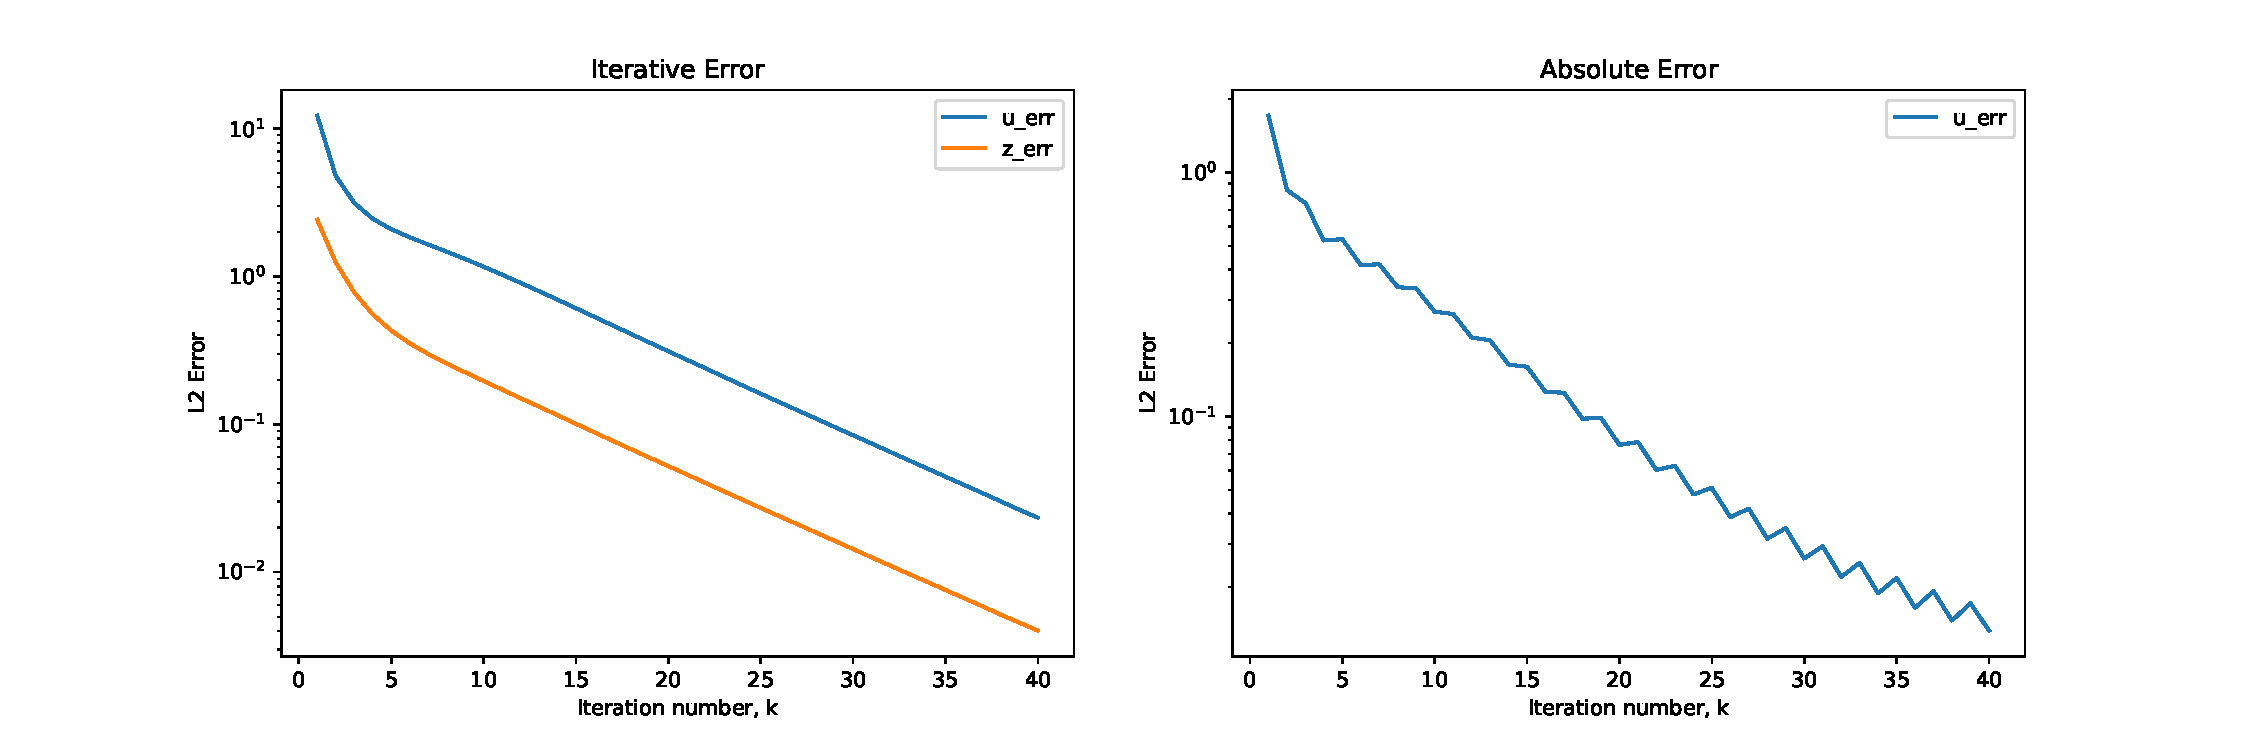
\includegraphics[width=0.9\textwidth]{error_plots_iii.pdf}
    \caption{Error plots, showing error in the $L^2([0,T],L^2(\Omega))$-norm. Left: the error between successive iterates $u^{(k)}-u^{(k-1)}$ and $z^{(k)}-z^{(k-1)}$. Right: the error between $u^{(k)}$, the current iterate, and the target $d_T$.}\label{fig:error-plots}
\end{figure}

In \autoref{fig:error-plots} we plot the iterative and absolute errors, $e_{IT}(k)$ and $e_{ABS}(k)$ versus the iteration number $k$. Both errors are plotted on a log-linear scale. We see that the iterative error looks like a straight line on this scale, which implies that convergence occurs in terms of a power law, i.e. that the error is proportional to $k^{n}$, for some number $n$. Meanwhile, the absolute error also looks approximately like a straight line on the log-linear scale. However, it's decreasing in a very jagged fashion, decreasing a lot more over one iteration in some cases than others, and even increasing slightly over one iteration in some cases.

We note that depending on the choice of $d_T$, in general the sought-after minimum might not, even in theory, be $u=d_T$. This could explain the fact that the absolute error does not seem to go to zero. Additionally, due to discretisation error, the values of the "true" optimum of the discretised optimisation problem and the values of the target function $d_T$ on the grid, will not be exactly equal for any finite discretisation. 

In this report, we have not gone into detail on the difference between the non-discretised optimisation problem and the discretised optimisation problem. In the field of PDE constrained optimisation, a distinction is often made between choosing to optimise (and thus, if the Lagrangian method is chosen, derive the coupled PDE system) first, and then discretising to solve the system numerically, or instead discretising first, and then optimising the discretised problem. For an in-detail discussion of this distinction, see e.g. \cite{rees_preconditioning_2010}. 

\section{Future work}
% \begin{itemize}
%     \item Show convergence of $(u^{(k)},z^{(k)})$ to the true solution $(u^{(*)},z^{(*)})$
%     \item Show convergence of $(u^{(k)},z^{(k)})$ to something (not neccessarily the true solution)
%     \item Extend our model to multiple dimensions in space
%     \item Consider other norms? FBSDE? 
%     \item Implement/find/come up with better numerical methods: e.g. Strong stability Preserving (SSP) methods, Multilevel Monte Carlo (MLMC), and maybe parallelize the Monte Carlo code (each "point" (t,x,v) could be run in parallel?) GPU or FPGA
% \end{itemize}

In this section, we discuss possible extensions of the material presented in this report, and outline some suggested directions for future work. First, we discuss showing convergence of the iterative procedure introduced in \autoref{sec:iterative-scheme}. Second, we discuss how the sensitivity of the convergence may be affected by the choice of methods and parameters for the numerical approximation of the PDE solutions. Then, we outline some possible ways to improve our current numerical methods. Finally, we discuss extensions of our current radiation transport model and optimisation problem.

It is not immediately clear whether the iterative scheme introduced in \autoref{sec:iterative-scheme} converges, whether if converges to the right thing, and if it does converge, in what sense it does so. One potential point of future work would be to firstly, show that the iterative scheme converges when considered in terms of the true (non-discretised) solutions to the PDEs for $u$ and $z$. This would amount to showing that $\lVert u^{(k)} - u^{(k-1)} \rVert$, goes to zero as $k$ goes to infinity, and similarly for $\lVert z^{(k)} - z^{(k-1)} \rVert$. Inspired by the results of the numerical experiment presented in \autoref{sec:numerical}, we theorize that this convergence should follow a power law, and suggest that a suitable norm to show convergence in might be the $L^2([0,T],L^2(\Omega))$-norm chosen for the optimisation problem. We would also want to show that $u^{(k)}$ and $z^{(k)}$ converge to the right thing, i.e. to the functions $u^{*}$ and $g^{*}$ which yield the minimum of \autoref{eq:to-minimise}. In this case, we'd want to show that $\lVert u^{(k)} - u^{*} \rVert$ and $\lVert \frac{1}{\alpha}z^{(k)} - g^{*} \rVert$ go to zero as $k$ goes to infinity.

After establishing convergence in the above case, we would want to consider how to establish convergence of the iterative procedure when it involves numerical approximations of $u^{(k)}$ and $z^{(k)}$ at each iteration. Relevant questions here include under what conditions the iterative procedure converges at all for the approximations of $u^{(k)}$ and $z^{(k)}$, and how close the functions it converges to are to the values at gridpoints of $u^{*}$ and $g^{*}$ defined above. We have an indication of the answer to the first of these questions from the results of the numerical experiement in \autoref{sec:numerical}. In more detail, the second question may be answered by investigating how the discretisation error (and in the case of $z^{(k)}$, Monte Carlo error) propagates through iterations. We also suggest investigating how the convergence rates of the respective numerical schemes for the primal and dual equations affect the closeness of (the approximation of) $u^{(k)}$ to $u^{*}$.

For the numerical simulations carried out in \autoref{sec:numerical}, we used a fairly simple finite difference scheme for the primal equation, and a straightforward Monte Carlo simulation based on an Euler-Maruyama discretisation for the dual equation. To improve upon the speed and accuracy of the algorithm, me may wish to consider both numerical methods with higher orders of convergence, and (on the Monte Carlo side) variance reduction techniques. For example, we could use a higher order finite difference scheme, as well as a higher order scheme (such as e.g. Milstein's scheme) to simulate the SDE. In terms of variance reduction techniques, we could apply a multilevel Monte Carlo (MLMC) technique -- see e.g. \cite{giles2008multilevel} or \cite{gobet2016monte}. As previously mentioned, for optimising the speed of our algorithm, we also recommend serialising the Monte Carlo simulations which yield the numerical approximation of $z^{(k)}$ across a grid in $t,x,v$, for each $k$. Inspiration can for example be taken from \cite{jia2012gpu}, where GPU accelerated Monte Carlo code is used for radiation dose calculations for proton beam therapy.

Additionally we may wish to specifically consider strong stability preserving numerical (SSP) methods, also known as total variation diminishing (TVD) methods, which preserve the monotonicity of a solution in space between timesteps. These methods are useful when simulating conservation laws or physical systems in general, as they yield numerical solutions that still obey the laws of physics. We refer to e.g. \cite{gottlieb2001strong}, \cite{gottlieb2005high} and \cite{harten1983upstream} for descriptions of SSP methods in the PDE setting, and to \cite{fang2023strong} for an SSP method formulated in the setting of FBSDE and nonlinear Feynman-Kac formulae. 

Finally, the radiation transport model \autoref{eq:pde-model} that has been considered in this report only features one spatial dimension. Since radiotherapy treatment naturally takes place in three dimensional space, a neccessary extension of our model for application in the real world, is extending the radiation model to three-dimensional space. We may also wish to further consider which norm it is most suitable to formulate the minimisation problem of \autoref{eq:to-minimise}. In the case where the choice of norm yields coupled nonlinear PDEs, e.g. those of \autoref{eq:nonlinear-pde-system}, we will then need to apply the theory of FBSDE and nonlinear Feynman-Kac formulae discussed in \autoref{sec:fbsde-theory} to obtain a probabilistic representation of the solution to the dual equation. We may also wish to apply the SSP methods for FBSDE from \cite{fang2023strong}, which we briefly outline in \autoref{sec:fbsde-numerics}.
\section{Summary and conclusion}
\begin{itemize}
    \item Summarize results and future work directions?
\end{itemize}

% \section{Spare Theory}

% - PDE Constrained optimisation problem 

% - Forward + Backward PDEs

% - Initial/terminal conditions, boundary conditions, and source terms (figure out equivalent formulations?)

% \vspace{5mm}
% - Forward + Backward SDEs

% - Connections between FBSDEs and the PDEs (eg distribution of process given by forward SDE is described by sol to Fokker-Planck/Kolmogorov forward eqn)

% - Feynman-Kac formulae (of various kinds)

% - Solving Fokker-Planck using MC + Feynman-Kac (as in reading course)

% - Simplest scheme for Forward-Backward SDEs

% - New (\cite{fang2023strong}) SSP scheme for FBSDEs

% - Specifically what schemes and equations look like for the reading course model

% - Similarities/Differences between the "first" (linear?) kind of Feynman-Kac formula, and the FBSDE *nonlinear* Feynman-Kac formulae?

% - CONSISTENT NOTATION --- there is something weird with functions $f$ and $g$ at the moment, for example\dots

% \bibliographystyle{plain}
% \bibliography{bibliography.bib}
\newpage
% \nocite{*}
\printbibliography
\end{document}
